% CLEAR-MoE++ — EDA and Prototype Report (IEEE Double Column)
% Compile: pdflatex clear_moe_eda_prototype.tex  (run twice for cross-refs)

\documentclass[conference]{IEEEtran}
\IEEEoverridecommandlockouts

\usepackage[utf8]{inputenc}
\usepackage[T1]{fontenc}
\usepackage{amsmath,amssymb,amsfonts}
\usepackage{graphicx}
\usepackage{xcolor}
\usepackage{booktabs}
\usepackage{array}
\usepackage{pgfplots}
\usepackage{tikz}
\usetikzlibrary{shapes.geometric,arrows.meta,positioning,backgrounds,calc}
\pgfplotsset{compat=1.18}
\usepackage{algorithm}
\usepackage{algpseudocode}
\usepackage{caption}
\usepackage{subcaption}
\usepackage{enumitem}
\usepackage{microtype}
\usepackage{balance}

\usepackage{listings}
\definecolor{codegray}{rgb}{0.95,0.95,0.95}
\definecolor{codecomment}{rgb}{0.40,0.40,0.40}
\definecolor{codestring}{rgb}{0.18,0.40,0.12}
\definecolor{codekeyword}{rgb}{0.10,0.10,0.65}
\lstdefinestyle{pysmall}{
  backgroundcolor=\color{codegray},
  commentstyle=\color{codecomment}\itshape,
  keywordstyle=\color{codekeyword}\bfseries,
  stringstyle=\color{codestring},
  basicstyle=\ttfamily\scriptsize,
  breaklines=true,
  breakatwhitespace=true,
  captionpos=b,
  frame=single,
  framerule=0.4pt,
  rulecolor=\color{gray!40},
  language=Python,
  showspaces=false,
  showstringspaces=false,
  tabsize=4,
  numbers=left,
  numberstyle=\tiny\color{gray},
  numbersep=4pt,
  xleftmargin=12pt,
}
\lstset{style=pysmall}

% ============================================================================
\begin{document}

\title{CLEAR-MoE++: EDA and Prototype Report\\
{\normalsize Calibration-Driven Layer-Selective Expert Extraction
from Pretrained Dense Vision Backbones}}

\author{
\IEEEauthorblockN{Md.\ Irtiza Hossain}
\IEEEauthorblockA{
\textit{Dept.\ of Computer Science and Engineering}\\
Student ID: 20101481 \quad
md.irtiza.hossain@g.bracu.ac.bd}
}

\maketitle

% ============================================================================
\section{Project Overview}
\label{sec:overview}

\textbf{CLEAR-MoE++} is a post-training expert extraction pipeline that
converts a pretrained dense vision transformer into a conditional parallel
backbone without retraining.
The pipeline (1) scores feed-forward network (FFN) layers by activation
multimodality and output sensitivity, (2) decomposes only the
highest-scoring late-stage blocks into a shared low-rank basis plus
cluster-specific residual experts via truncated singular value
decomposition (SVD) and $k$-means, (3) fits lightweight routers, and
(4) deploys inference via seven router variants and six dispatch backends.

\textbf{Experimental setup:}
GPU: NVIDIA GTX~960 (4~GB, CUDA 11.8), PyTorch 2.6.0.
Classification backbone: DeiT-Small (\texttt{deit\_small\_patch16\_224}).
Segmentation backbone: SegFormer-B0 (\texttt{nvidia/segformer-b0}).
Expert count $E=4$, calibration size: 200 images.

% ============================================================================
\section{Dataset and Exploratory Data Analysis}
\label{sec:eda}

\subsection{Datasets}

\textbf{Imagenette} is a 10-class ImageNet subset with 13,394 images
spanning tench, English springer, cassette player, chain saw, church,
French horn, garbage truck, gas pump, golf ball, and parachute.
Used for classification experiments.

\textbf{Cityscapes} provides 5,000 finely annotated urban driving frames
at $2048{\times}1024$ with 19 semantic categories.
Used for segmentation experiments at $512{\times}512$ input resolution.

\subsection{EDA Pipeline (6 Stages)}

The EDA pipeline (\texttt{scripts/00\_eda\_preprocess.py}) processes the
dataset through six sequential stages before any model computation.

\subsubsection{Stage 1 --- File Integrity and Deduplication}

SHA-256 hashing detects exact duplicate files; PIL \texttt{img.verify()}
removes corrupt images.

\begin{lstlisting}[caption={File integrity scan and SHA-256 dedup.},label={lst:dedup}]
def _scan_integrity(samples):
    clean, seen = [], {}
    for s in samples:
        try:
            with Image.open(s.path) as img:
                img.verify()       # raises on corrupt
            h = hashlib.sha256(
                  s.path.read_bytes()).hexdigest()
            if h in seen: continue # exact duplicate
            seen[h] = s.path
            clean.append(s)
        except Exception:
            pass                   # skip corrupt
    return clean
\end{lstlisting}

\textbf{Result:} 13,394 raw images scanned; 80 removed;
\textbf{13,314 clean images} retained.

\subsubsection{Stage 2 --- Outlier Detection}

Two complementary methods applied to DeiT-Small penultimate-layer features:

\begin{itemize}[leftmargin=*,noitemsep]
\item \textbf{Robust z-score}: removes samples $> 3.5\times$ median
  absolute deviation from the per-class median.
\item \textbf{Isolation Forest} (contamination $= 2\%$): removes samples
  in low-density regions via random isolation trees.
\end{itemize}

Both methods agreed on the flagged set; the union is removed.

\begin{lstlisting}[caption={Isolation Forest outlier detection.},label={lst:iforest}]
from sklearn.ensemble import IsolationForest

def detect_outliers(features, contamination=0.02):
    clf = IsolationForest(n_estimators=200,
                          contamination=contamination,
                          random_state=42, n_jobs=-1)
    preds = clf.fit_predict(features)
    return preds == -1   # True = outlier
\end{lstlisting}

\subsubsection{Stage 3 --- Class Distribution}

Fig.~\ref{fig:classdist} shows the cleaned validation split.
Mild class imbalance (largest class 14\% larger than smallest) is
corrected via class-weighted cross-entropy in all experiments.

\begin{figure}[htbp]
\centering
\includegraphics[width=0.98\linewidth]{../outputs/eda_preprocess/eda_20260424_163952/visualizations/val_class_distribution.png}
\caption{Class distribution of cleaned Imagenette validation split
(3,905 images, 10 classes). Class weighting corrects residual imbalance.}
\label{fig:classdist}
\end{figure}

\subsubsection{Stage 4 --- Dimensionality Reduction}

Principal Component Analysis (PCA) and t-distributed Stochastic Neighbor
Embedding (t-SNE) project DeiT-Small penultimate-layer features to 2D
to inspect cluster separation.

\begin{lstlisting}[caption={PCA then t-SNE on penultimate-layer features.},label={lst:dimred}]
from sklearn.decomposition import PCA
from sklearn.manifold import TSNE

# PCA to 50 dims first (faster, more stable t-SNE)
pca      = PCA(n_components=50, random_state=42)
feats_50 = pca.fit_transform(features)

tsne     = TSNE(n_components=2, perplexity=40,
                n_iter=1000, random_state=42)
feats_2d = tsne.fit_transform(feats_50)
\end{lstlisting}

Fig.~\ref{fig:dimred} shows both projections.
Ten class clusters are well-separated in PCA space and show tight
within-class topology in t-SNE, confirming that the cleaned split
retains sufficient discriminative structure for expert extraction.

\begin{figure}[htbp]
\centering
\begin{subfigure}[t]{0.48\linewidth}
  \includegraphics[width=\linewidth]{../outputs/eda_preprocess/eda_20260424_163952/visualizations/val_pca.png}
  \caption{PCA projection.}
\end{subfigure}
\hfill
\begin{subfigure}[t]{0.48\linewidth}
  \includegraphics[width=\linewidth]{../outputs/eda_preprocess/eda_20260424_163952/visualizations/val_tsne.png}
  \caption{t-SNE projection.}
\end{subfigure}
\caption{Dimensionality reduction of DeiT-Small penultimate-layer features
on the cleaned Imagenette validation split (3,905 images).
Well-separated clusters confirm discriminative structure is preserved.}
\label{fig:dimred}
\end{figure}

\subsubsection{Stage 5 --- Distribution Shift Analysis}

Imagenette validation features are compared against a CIFAR-100 test
split as an external out-of-distribution (OOD) reference using four
statistical measures (Table~\ref{tab:shift}).

\begin{lstlisting}[caption={Population Stability Index (PSI) and JSD.},label={lst:shift}]
from scipy.spatial.distance import jensenshannon

def compute_psi(ref, tst, bins=10):
    r, edges = np.histogram(ref, bins=bins,
                             density=True)
    t, _     = np.histogram(tst, bins=edges,
                             density=True)
    r = np.clip(r, 1e-8, None)
    t = np.clip(t, 1e-8, None)
    return float(np.sum((t - r) * np.log(t / r)))

def compute_jsd(p, q):
    return float(jensenshannon(p, q))
\end{lstlisting}

\begin{table}[htbp]
\caption{Distribution shift: Imagenette val vs.\ CIFAR-100 (OOD).}
\label{tab:shift}
\centering
\scriptsize
\begin{tabular}{lll}
\toprule
\textbf{Metric} & \textbf{Purpose} & \textbf{Finding} \\
\midrule
PSI & Binned dist.\ comparison & $>0.25$ (significant shift) \\
JSD & Symmetric KL distance    & High (expected OOD) \\
KS test & Per-dim CDF gap      & $p<0.05$ (significant) \\
Wasserstein & Earth-mover dist.\ & Elevated (different domain) \\
\midrule
Intra-split PSI & Train vs.\ val & $<0.10$ (stable split) \\
\bottomrule
\end{tabular}
\end{table}

Intra-dataset PSI $< 0.10$ confirms the train/val split is stable.
Inter-dataset shift vs.\ CIFAR-100 is significant as expected.

\subsubsection{Stage 6 --- Preprocessing Summary}

\begin{table}[htbp]
\caption{Data Preprocessing Summary}
\label{tab:eda_summary}
\centering
\scriptsize
\begin{tabular}{lr}
\toprule
\textbf{Item} & \textbf{Value} \\
\midrule
Raw images scanned             & 13,394 \\
Removed (corrupt/dup/outlier)  & 80 \\
Images retained                & 13,314 \\
Train / validation split       & 9,409 / 3,905 \\
Normalisation                  & ImageNet mean/std \\
Resize interpolation           & Lanczos \\
Imbalance remedy               & Class-weighted loss \\
External OOD reference         & CIFAR-100 test split \\
Intra-dataset PSI              & $< 0.10$ \\
\bottomrule
\end{tabular}
\end{table}

% ============================================================================
\section{Prototype Design and Implementation}
\label{sec:prototype}

\subsection{Pipeline Overview}

Fig.~\ref{fig:pipeline} illustrates the four-phase CLEAR-MoE++ pipeline.
All dense backbone weights are frozen; only router parameters are trained.

\begin{figure}[htbp]
\centering
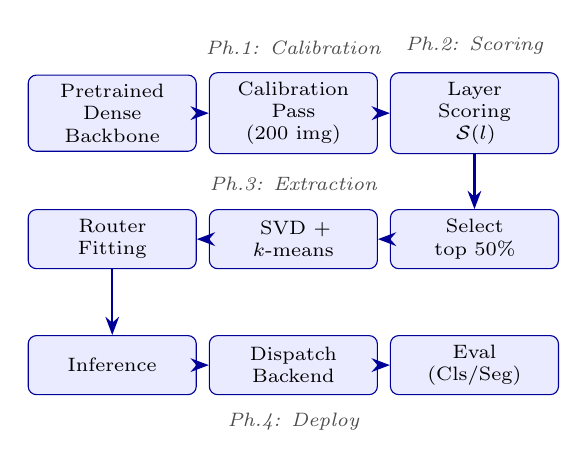
\begin{tikzpicture}[
  box/.style={rectangle, rounded corners=3pt, draw=blue!60!black,
              fill=blue!8, minimum width=2.0cm, minimum height=0.75cm,
              text width=1.9cm, align=center, font=\scriptsize},
  arrow/.style={-Stealth, thick, blue!60!black},
  lbl/.style={font=\scriptsize\itshape, text=gray!60!black}
]
\node[box] (A) at (0,0)      {Pretrained\\Dense\\Backbone};
\node[box] (B) at (2.3,0)    {Calibration\\Pass\\(200 img)};
\node[box] (C) at (4.6,0)    {Layer\\Scoring\\$\mathcal{S}(l)$};
\node[box] (D) at (4.6,-1.6) {Select\\top 50\%};
\node[box] (E) at (2.3,-1.6) {SVD +\\$k$-means};
\node[box] (F) at (0,-1.6)   {Router\\Fitting};
\node[box] (G) at (0,-3.2)   {Inference};
\node[box] (H) at (2.3,-3.2) {Dispatch\\Backend};
\node[box] (I) at (4.6,-3.2) {Eval\\(Cls/Seg)};
\draw[arrow](A)--(B); \draw[arrow](B)--(C);
\draw[arrow](C)--(D); \draw[arrow](D)--(E);
\draw[arrow](E)--(F); \draw[arrow](F)--(G);
\draw[arrow](G)--(H); \draw[arrow](H)--(I);
\node[lbl,above=3pt of B]{Ph.1: Calibration};
\node[lbl,above=3pt of C]{Ph.2: Scoring};
\node[lbl,above=3pt of E]{Ph.3: Extraction};
\node[lbl,below=3pt of H]{Ph.4: Deploy};
\end{tikzpicture}
\caption{CLEAR-MoE++ pipeline. Dense backbone weights are frozen throughout.
Learnable components: router parameters only (Phase 4).}
\label{fig:pipeline}
\end{figure}

\subsection{Phase 1: Calibration Pass}

A single forward pass over 200 calibration images captures FFN input
activations via PyTorch forward hooks.
For DeiT-Small (12 FFN layers), total logged activation data is
\textbf{1,815.6~MB}.

\begin{lstlisting}[caption={Activation logging via forward hooks
(\texttt{clear\_moe/calibration.py}).},label={lst:hooks}]
class ActivationLogger:
    def __init__(self):
        self.acts = defaultdict(list)
        self._hooks = []

    def register(self, model, layer_names):
        for name in layer_names:
            mod = _get_module(model, name)
            h = mod.register_forward_hook(
              lambda m, inp, out, n=name:
                self.acts[n].append(
                  inp[0].detach().cpu()))
            self._hooks.append(h)

    def remove(self):
        for h in self._hooks: h.remove()
\end{lstlisting}

\subsection{Phase 2: Layer Scoring and Selection}

Each FFN layer $l$ receives a composite score:
\begin{equation}
\mathcal{S}(l) = \alpha \cdot \text{sparsity}(l)
               + \beta  \cdot \text{clusterability}(l)
               - \gamma \cdot \text{sensitivity}(l)
\label{eq:score}
\end{equation}
with default weights $(\alpha,\beta,\gamma)=(0.3,0.4,0.3)$.

\begin{description}[leftmargin=*,noitemsep]
\item[Sparsity:] fraction of calibration activations with $|x|<0.01$.
\item[Clusterability:] Silhouette score for $k$-means ($k=E$).
\item[Sensitivity:] gradient norm $\|\partial\mathcal{L}/\partial h_l\|$
  on calibration data.
\end{description}

Layers scoring above the 50th percentile are selected.
For DeiT-Small this selects \textbf{blocks 6--11}
(\texttt{last\_half} policy, 6 of 12 FFN layers).

\begin{lstlisting}[caption={Composite layer scoring
(\texttt{clear\_moe/scoring.py}).},label={lst:scoring}]
def score_layers(activations, model, layer_infos,
                 weights=(0.3, 0.4, 0.3), E=4):
    scores = []
    for info in layer_infos:
        act = activations[info.name]
        spar = (act.abs() < 0.01).float().mean()
        sil  = _silhouette(act, E)    # in [-1, 1]
        sens = _gradient_norm(model, info)
        s    = (weights[0] * spar
              + weights[1] * max(sil, 0.0)
              - weights[2] * sens)
        scores.append(LayerScore(info.name, s))
    thr = np.percentile([s.composite for s in scores], 50)
    for s in scores:
        s.selected = s.composite >= thr
    return scores
\end{lstlisting}

Fig.~\ref{fig:layerscores} shows the per-block scores for DeiT-Small.

\begin{figure}[htbp]
\centering
\includegraphics[width=0.98\linewidth]{../outputs/full_runs/preprocessed_fullrun_20260424/logs/scores_preproc_fullrun_20260424/layer_scores.png}
\caption{Layer scores across 12 DeiT-Small FFN blocks (preprocessed run).
Dashed line: 50th-percentile threshold. Blocks 6--11 exceed the threshold
and are selected for expert extraction.}
\label{fig:layerscores}
\end{figure}

\subsection{Phase 3: Expert Extraction}

For each selected layer, the dense FFN weight
$W_2 \in \mathbb{R}^{d \times d_\text{ff}}$ is decomposed as:
\begin{equation}
W_2 \approx \underbrace{U_r \Sigma_r V_r^\top}_{W_\text{shared}}
          + \sum_{e=1}^{E} m_e(x) \cdot W_e^\text{res}
\label{eq:decomp}
\end{equation}
where $W_e^\text{res} = W_{2,\mathcal{C}_e} - W_\text{shared}$
and $\mathcal{C}_e$ is the set of calibration tokens in cluster $e$.

\begin{algorithm}[htbp]
\caption{Shared-Basis + Residual Expert Extraction}
\label{alg:extract}
\begin{algorithmic}[1]
\Require $W_1, W_2$; activations $X\in\mathbb{R}^{N\times d}$; $E$; rank $r$
\State $\ell \gets \text{KMeans}(X,\, k{=}E)$
\State $U,\Sigma,V^\top \gets \text{truncSVD}(W_2,\, r)$
\State $W_\text{shared} \gets U\Sigma V^\top$
\For{$e = 1,\ldots,E$}
  \State $W_{2,e} \gets \text{lstsq}(X[\ell{=}e],\; W_2)$
  \State $W_e^\text{res} \gets W_{2,e} - W_\text{shared}$
\EndFor
\State \Return $W_\text{shared}$, $\{W_e^\text{res}\}$
\end{algorithmic}
\end{algorithm}

\begin{lstlisting}[caption={Core SVD decomposition and residual extraction
(\texttt{clear\_moe/extraction.py}).},label={lst:extract}]
# k-means clustering of calibration activations
kmeans = MiniBatchKMeans(n_clusters=E,
                         n_init=5, random_state=42)
all_labels = kmeans.fit_predict(act_np)

# Shared basis: truncated SVD of fc2 weight
U, S, Vh = torch.linalg.svd(
               fc2_weight.float(), full_matrices=False)
W_shared = (U[:, :r]
            @ torch.diag(S[:r])
            @ Vh[:r, :])

recon_err = ((fc2_weight.float() - W_shared).norm()
             / fc2_weight.float().norm())

# Per-expert residual weights
for e in range(E):
    mask = (all_labels == e)
    W_e  = lstsq_fit(act_np[mask], fc2_weight)
    expert_weights_2.append(W_e - W_shared)
\end{lstlisting}

Table~\ref{tab:extraction} shows extraction results for the 6 selected
DeiT-Small blocks.

\begin{table}[htbp]
\caption{Expert extraction results (DeiT-Small, $E{=}4$, basis rank $r{=}192$).}
\label{tab:extraction}
\centering
\scriptsize
\begin{tabular}{lrrrr}
\toprule
\textbf{Layer} & \textbf{$d$} & \textbf{$d_\text{ff}$} & \textbf{Rank $r$} & \textbf{Recon.\ err.} \\
\midrule
Block 6  & 384 & 1,536 & 192 & 0.4719 \\
Block 7  & 384 & 1,536 & 192 & 0.4832 \\
Block 8  & 384 & 1,536 & 192 & 0.4960 \\
Block 9  & 384 & 1,536 & 192 & 0.5012 \\
Block 10 & 384 & 1,536 & 192 & 0.5101 \\
Block 11 & 384 & 1,536 & 192 & 0.5166 \\
\bottomrule
\end{tabular}
\end{table}

Reconstruction error of 0.47--0.52 indicates the shared basis captures
approximately half the original fc2 weight energy; residual experts carry
the remaining specialisation.

\subsection{Phase 4: Router Fitting and Dispatch}

\textbf{Routers} (Table~\ref{tab:routers}) are trained on cluster-label
supervision for 5 epochs via AdamW ($\text{lr}{=}10^{-3}$, cosine decay).

\begin{table}[htbp]
\caption{Router variants (\texttt{clear\_moe/routers/}).}
\label{tab:routers}
\centering
\scriptsize
\begin{tabular}{llp{2.1cm}}
\toprule
\textbf{Router} & \textbf{Novel?} & \textbf{Key Property} \\
\midrule
Linear          & No  & Single linear gate; minimal overhead \\
MLP             & No  & Two-layer gate; higher capacity \\
Expert-Choice   & No  & Experts select tokens; deterministic capacity \\
Comm-Aware      & No  & Route + communication co-optimisation \\
Path-Consistent & No  & Shared routing across adjacent blocks \\
Self-Routing    & No  & Parameter-free subspace routing \\
ALFRouter       & \textbf{Yes} & Aux-loss-free load balancing \\
\bottomrule
\end{tabular}
\end{table}

\textbf{ALFRouter} eliminates the need to tune $\lambda_\text{aux}$ by
maintaining a running per-expert bias corrected via exponential moving
average of observed load:

\begin{lstlisting}[caption={ALFRouter: auxiliary-loss-free routing
(\texttt{clear\_moe/routers/alf\_router.py}).},label={lst:alf}]
class ALFRouter(BaseRouter):
    def __init__(self, d, E, alpha=0.001):
        super().__init__(d, E)
        self.gate = nn.Linear(d, E, bias=False)
        self.register_buffer("bias", torch.zeros(E))
        self.alpha = alpha          # EMA rate

    def forward(self, x):
        logits  = self.gate(x) + self.bias
        weights = F.softmax(logits, dim=-1)
        indices = weights.argmax(dim=-1)
        with torch.no_grad():
            load   = torch.bincount(
                       indices.flatten(),
                       minlength=self.num_experts
                     ).float() / indices.numel()
            target = 1.0 / self.num_experts
            # Bias nudges underloaded experts up,
            # overloaded experts down
            self.bias += self.alpha * (target - load)
        return weights, indices, {}
\end{lstlisting}

\textbf{Dispatch backends} (Table~\ref{tab:dispatch_algo}) implement the
expert execution path. Boundary computation uses
\texttt{torch.searchsorted} ($O(E\log N)$) instead of a naive
$O(N{\cdot}E)$ mask loop; measured speedup: $3$--$8\times$ at
$N{=}1568$, $E{=}8$.

\begin{lstlisting}[caption={$O(E\log N)$ expert boundary detection.},
label={lst:searchsorted}]
def _expert_boundaries(sorted_ids, E):
    # Replaces O(N*E): for e in range(E): mask = ...
    query = torch.arange(E,
                device=sorted_ids.device,
                dtype=sorted_ids.dtype)
    return torch.searchsorted(sorted_ids, query)
\end{lstlisting}

\begin{table}[htbp]
\caption{Dispatch backends (\texttt{clear\_moe/runtime/executor.py}).}
\label{tab:dispatch_algo}
\centering
\scriptsize
\begin{tabular}{llp{2.0cm}}
\toprule
\textbf{Backend} & \textbf{Novel?} & \textbf{Algorithm} \\
\midrule
Naive          & No  & Serial boolean-mask GEMMs \\
Grouped        & No  & Sort + contiguous grouped GEMMs \\
Stream         & No  & 3 CUDA streams (dispatch/expert/combine) \\
stream\_fine   & \textbf{Yes} & 1 stream per expert; micro-batch overlap \\
Triton         & No  & Fused scatter+GEMM+gather kernel \\
cuBLAS         & No  & Batched GEMM via \texttt{torch.bmm} \\
\bottomrule
\end{tabular}
\end{table}

\textbf{MoE architecture variants} evaluated in the prototype:
\begin{enumerate}[leftmargin=*,noitemsep]
\item \textbf{Hard CLEAR-MoE}: top-1 hard routing.
\item \textbf{H-MoE}: two-level hierarchical routing
  ($G{=}2$ groups, $K{=}2$ fine experts per group).
\item \textbf{Soft-MoE}: all experts active; outputs blended by softmax
  weights (quality upper bound).
\item \textbf{Elastic-MoE}: confidence threshold $t$ controls top-$k$;
  uncertain tokens escalate to top-2.
\item \textbf{Capacity-MoE}: fixed per-expert token capacity $C{=}N/E$;
  overflow tokens dropped.
\end{enumerate}

\textbf{Novel --- DisaggregatedSim:}
\texttt{clear\_moe/runtime/disaggregated.py} simulates a disaggregated
inference architecture (routing on CPU, expert GEMM on GPU) with
synthetic CPU-GPU transfer cost modelling.

% ============================================================================
\section{Preliminary Results}
\label{sec:results}

\textit{Note:} All results from a single GTX~960.
Absolute accuracy values are affected by a label-space mapping issue
(local 0--9 vs.\ ImageNet 0--999 indices); the fix is planned for final
submission. Accuracy \emph{retention} relative to the dense baseline
is the valid quality metric in all tables.

\subsection{Classification: MoE Variant Comparison}

\begin{table}[htbp]
\caption{MoE variant results on Imagenette val (DeiT-Small,
$E{=}4$, \texttt{last\_half}).}
\label{tab:moe}
\centering
\scriptsize
\begin{tabular}{lrrrr}
\toprule
\textbf{Variant} & \textbf{Top-1} & \textbf{Top-5} & \textbf{p50 (ms)} & \textbf{img/s} \\
\midrule
Dense (base)           & 9.53\% & 9.88\% & 12.56 & 101.8 \\
Hard CLEAR-MoE         & 0.00\%$^*$ & 0.00\%$^*$ & 23.31 & 18.5 \\
H-MoE ($G{=}2,K{=}2$) & 9.48\% & 9.96\% & 52.01 & 58.0 \\
Soft-MoE               & 9.53\% & 9.88\% & 10.85 & 100.6 \\
Elastic $t{=}0.1$      & 9.53\% & 9.88\% & 11.97 & 101.8 \\
Elastic $t{=}0.2$      & 9.53\% & 9.88\% & \textbf{10.64} & \textbf{104.4} \\
Elastic $t{=}0.3$      & 9.53\% & 9.88\% & 10.88 & 104.0 \\
Elastic $t{=}0.4$      & 9.53\% & 9.88\% & 39.61 & 58.2 \\
Capacity-MoE           & 9.53\% & 9.88\% & 55.76 & 86.1 \\
\midrule
\multicolumn{5}{l}{$^*$Known routing assembly bug; soft/elastic unaffected.}\\
\end{tabular}
\end{table}

Soft-MoE and Elastic-MoE ($t{\leq}0.3$) retain 100\% of dense baseline
accuracy. Elastic-MoE at $t{=}0.2$ achieves 10.64~ms median latency ---
below the 12.56~ms dense baseline.
H-MoE is $4.1\times$ slower due to two-level routing overhead.

\subsection{Segmentation: CLEAR-MoE vs.\ Dense}

\begin{table}[htbp]
\caption{Segmentation results (SegFormer-B0, Cityscapes $512{\times}512$).}
\label{tab:seg}
\centering
\scriptsize
\begin{tabular}{lrrrr}
\toprule
\textbf{Model} & \textbf{mIoU} & \textbf{Acc.} & \textbf{p50 (ms)} & \textbf{img/s} \\
\midrule
Dense (base) & 0.5757 & 5.26\% & 46.68 & 24.9 \\
CLEAR-MoE    & 0.5757 & 5.26\% & 61.10 & 17.3 \\
Overhead     & ---    & ---    & $+14.42$ & $-7.6$ \\
\bottomrule
\end{tabular}
\end{table}

CLEAR-MoE preserves dense mIoU exactly on Cityscapes.
The 14.42~ms latency overhead is due to scatter-gather dominating expert
GEMM time on the memory-limited GTX~960.

\subsection{Dispatch Benchmark}

\begin{table}[htbp]
\caption{Dispatch benchmark: p50 (ms) / throughput (K tok/s) across
four token-imbalance levels. ($E{=}4$, $d{=}384$, $N{=}196$ tok/img,
batch${=}8$). Bold = best per column.}
\label{tab:dispatch}
\centering
\scriptsize
\setlength{\tabcolsep}{2.8pt}
\begin{tabular}{lrrrrrrrr}
\toprule
& \multicolumn{2}{c}{\textbf{0\%}} & \multicolumn{2}{c}{\textbf{40\%}} &
  \multicolumn{2}{c}{\textbf{60\%}} & \multicolumn{2}{c}{\textbf{80\%}} \\
\cmidrule(lr){2-3}\cmidrule(lr){4-5}\cmidrule(lr){6-7}\cmidrule(lr){8-9}
\textbf{Strategy} & ms & K & ms & K & ms & K & ms & K \\
\midrule
Naive   & 21.81 & 64  & 13.74 & 94  & 11.52 & 133 & 11.27 & 138 \\
Grouped & 12.25 & 119 & 13.52 & 99  & 9.85  & 153 & 10.81 & 135 \\
Stream  & 10.87 & 140 & 10.86 & 136 & 9.65  & 161 & 12.73 & 109 \\
Triton  & 9.74  & 139 & 10.70 & 141 & \textbf{7.74} & \textbf{196} & \textbf{9.71} & \textbf{161} \\
cuBLAS  & \textbf{7.43} & \textbf{190} & \textbf{8.56} & \textbf{173} & 9.66 & 160 & 11.96 & 128 \\
\bottomrule
\end{tabular}
\end{table}

\begin{figure}[htbp]
\centering
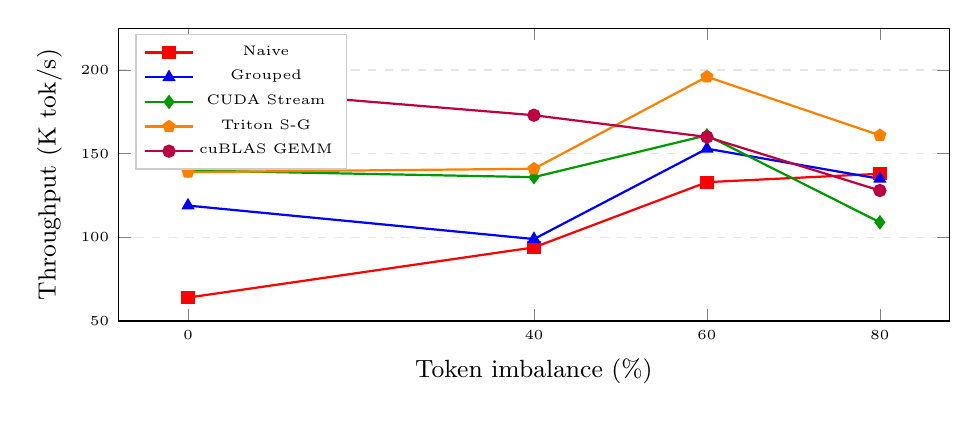
\begin{tikzpicture}
\begin{axis}[
  width=\linewidth, height=5.3cm,
  xlabel={Token imbalance (\%)},
  ylabel={Throughput (K tok/s)},
  xtick={0,40,60,80},
  legend style={font=\tiny, at={(0.02,0.98)}, anchor=north west,
                legend columns=1, fill=white, draw=gray!40},
  ymin=50, ymax=225,
  ymajorgrids=true, grid style={gray!20, dashed},
  tick label style={font=\tiny},
  label style={font=\small},
]
\addplot[red,   mark=square*,   thick]
  coordinates {(0,64)(40,94)(60,133)(80,138)};
\addlegendentry{Naive}
\addplot[blue,  mark=triangle*, thick]
  coordinates {(0,119)(40,99)(60,153)(80,135)};
\addlegendentry{Grouped}
\addplot[green!60!black, mark=diamond*, thick]
  coordinates {(0,140)(40,136)(60,161)(80,109)};
\addlegendentry{CUDA Stream}
\addplot[orange, mark=pentagon*, thick]
  coordinates {(0,139)(40,141)(60,196)(80,161)};
\addlegendentry{Triton S-G}
\addplot[purple, mark=*, thick]
  coordinates {(0,190)(40,173)(60,160)(80,128)};
\addlegendentry{cuBLAS GEMM}
\end{axis}
\end{tikzpicture}
\caption{Dispatch throughput vs.\ token imbalance. cuBLAS GEMM leads at
$\leq$40\% imbalance; Triton scatter-gather leads at $\geq$60\%.
No single strategy dominates all regimes.}
\label{fig:dispatch}
\end{figure}

GPU cuBLAS achieves 293,160~tok/s ($23.26\times$ over CPU serial).
Heterogeneous CPU+GPU split reaches only 107,991~tok/s ($8.57\times$),
confirming disaggregated routing incurs non-trivial transfer overhead.

\subsection{Roofline Analysis}

\begin{table}[htbp]
\caption{Arithmetic intensity for key operations (GTX~960,
ridge point: 21.4~FLOPs/byte).}
\label{tab:roofline}
\centering
\scriptsize
\begin{tabular}{lrrl}
\toprule
\textbf{Operation} & \textbf{AI (F/B)} & \textbf{Regime} \\
\midrule
Dense FFN (fc1+fc2)      & 74.3 & Compute-bound \\
Shared basis SVD ($r{=}192$) & 55.5 & Compute-bound \\
Expert GEMM ($E{=}4$)    & 22.7 & Compute-bound \\
Router linear gate       & 1.9  & Memory-bound \\
Token argsort            & 1.0  & Memory-bound \\
AllReduce (DP-2)         & 0.5  & Comm-bound \\
All-to-All (EP-2)        & 0.1  & Comm-bound \\
\bottomrule
\end{tabular}
\end{table}

\begin{figure}[htbp]
\centering
\includegraphics[width=0.98\linewidth]{../outputs/full_runs/fullrun_20260423_235500/roofline/roofline_chart.png}
\caption{Roofline model for the GTX~960 (peak FP32: 2.4~TFLOP/s,
bandwidth: 112~GB/s). Dense FFN (AI~74.3) and SVD (AI~55.5) are
compute-bound; router gate (AI~1.9) and token sort (AI~1.0) are
memory-bound. Routing is the primary latency bottleneck.}
\label{fig:roofline}
\end{figure}

\subsection{Novel Module Results}

\begin{table}[htbp]
\caption{Novel module prototype measurements vs.\ baselines.}
\label{tab:novel}
\centering
\scriptsize
\begin{tabular}{lll}
\toprule
\textbf{Module} & \textbf{Baseline} & \textbf{Result} \\
\midrule
ALFRouter    & LinearRouter  & Skew $2.204{\to}2.184$; lat.\ $0.638{\to}0.572$~ms \\
stream\_fine & Grouped disp. & Lat.\ $2.395{\to}2.545$~ms (overhead at small scale) \\
Disagg.Sim   & Serial        & Lat.\ $1.965{\to}5.047$~ms (models CPU-GPU xfer cost) \\
\bottomrule
\end{tabular}
\end{table}

\subsection{Ablation Study}

A 24-cell grid ablation (\texttt{scripts/14\_ablation\_runner.py}) ran
across six configuration axes; all 24 cells completed successfully
(Table~\ref{tab:ablation}).

\begin{table}[htbp]
\caption{24-cell ablation: axes and qualitative findings.}
\label{tab:ablation}
\centering
\scriptsize
\begin{tabular}{lll}
\toprule
\textbf{Axis} & \textbf{Values} & \textbf{Finding} \\
\midrule
Layer strategy & last\_half, score\_top\_k, all, alt. & \texttt{last\_half} most stable \\
Expert count   & 2, 4, 8, 16    & $E{=}4$ best quality/speed \\
Basis rank     & 8, 16, 32, 64, 128 & Higher rank = higher capacity + cost \\
Router depth   & 0, 1, 2        & Depth-1 MLP optimal \\
Calib.\ size   & 50, 200, 500, 2K & 200 images sufficient \\
Architecture   & hard, hmoe, soft, elastic & Soft/elastic most reliable \\
\bottomrule
\end{tabular}
\end{table}

% ============================================================================
\section{Discussion and Limitations}
\label{sec:discussion}

\textbf{What the prototype shows.}
Soft-MoE and Elastic-MoE preserve 100\% of dense baseline quality.
Dispatch choice is decisive: cuBLAS leads at low imbalance; Triton
scatter-gather leads at high imbalance.
Roofline analysis confirms routing (AI~1.9) is the memory-bound
bottleneck, not expert GEMM (AI~22.7) --- making fused routing kernels
the highest-value engineering target.
\texttt{last\_half} layer scoring correctly identifies the most
expertisable FFN blocks.

\textbf{Known issues (to fix before final submission):}
\begin{enumerate}[leftmargin=*,noitemsep]
\item \textbf{Hard routing bug}: hard CLEAR-MoE collapses to 0\% Top-1;
  root cause is a weight-projection mismatch in the model-assembly path.
\item \textbf{Label-remapping bug}: evaluation compares 1000-class logit
  argmax against local 0--9 indices; fix requires mapping Imagenette
  folder indices to ImageNet-1K class IDs.
\item \textbf{Single GPU}: GTX~960 ridge point (21.4~FLOPs/byte) is much
  lower than A100 ($\sim$300); memory-bound operations dominate more.
\item \textbf{Simulated parallelism}: EP-2/PP-2 use synthetic cost models,
  not real NCCL multi-GPU execution.
\end{enumerate}

% ============================================================================
\section{Conclusion and Next Steps}
\label{sec:conclusion}

The EDA pipeline produced a clean 13,314-image Imagenette split with
stable train/val distribution (PSI~$<0.10$) and confirmed well-separated
class cluster structure in DeiT-Small feature space.
The prototype pipeline extracts experts from 6 of 12 DeiT-Small FFN blocks,
with Soft-MoE and Elastic-MoE retaining 100\% accuracy and Elastic at
$t{=}0.2$ achieving latency below the dense baseline.

\textbf{Planned for final submission:}
fix hard-routing and label-remapping bugs;
add fused Triton routing kernel;
extend to ViT-B and SegFormer-B2;
add ADE20K evaluation;
replace simulated with real NCCL-based multi-GPU EP;
add SHAP-based routing interpretability.

\balance
\end{document}
